\section{Visibility and Life-cycle of Variables}
\label{sec:vars}
\begin{frame}<beamer>
    \frametitle{Outline}
    \tableofcontents[currentsection]
\end{frame}

\begin{frame}[fragile]{Visibility and Life-cycle of Variables (1)}
\begin{itemize}
	\item {We take something for granted before}
	\item {Now we study them in detail}
	\begin{enumerate}
		\item {Could we use the same variable name in different functions?}
		\item {Could we use the same variable name in the same functions?}
		\item {Could different functions share the same variable?}
		\item {When a variable is born, when it dies??}
	\end{enumerate}
\end{itemize}

\end{frame}

\begin{frame}[fragile]{Visibility and Life-cycle of Variables (2)}
\begin{enumerate}
	\item {Could we use the same variable name in different functions?}
\end{enumerate}
\begin{columns}
\begin{column}{0.53\linewidth}
\begin{lstlisting}[linewidth=0.9\linewidth, xleftmargin=0.05\linewidth]
int func1(int n)
{
   int r = 3, a = 1;
   return (r*n+a);
}
float func2(int n, float a)
{
   float r = 1;
   int i = 0;
   for(i = 0; i < n; i++)
   {
      r = r*a;
   }
   return r;
}
\end{lstlisting}
\end{column}
\begin{column}{0.46\linewidth}
\begin{itemize}
	\item {The answer is \textcolor{red}{Yes}}
	\item {The visibility is inside function only}
	\item {It is born when the function is called}
	\item {It dies when calling is done}
\end{itemize}
\end{column}
\end{columns}
\end{frame}

\begin{frame}[fragile]{Visibility and Life-cycle of Variables (3)}
\begin{enumerate}
	\setcounter{enumi}{1}
	\item {Could we use the same variable name in the same function?}
\end{enumerate}
\begin{columns}
\begin{column}{0.55\linewidth}
\begin{lstlisting}[linewidth=0.9\linewidth, xleftmargin=0.05\linewidth]
float func2(int n, float a)
{
  float r = 1;
  int r = 0;
  int i = 0;
  float i = 0;
  for(i = 0; i < n; i++, r++)
  {
     r = r*a;
  }
  return r;
}
\end{lstlisting}
\end{column}
\begin{column}{0.44\linewidth}
\begin{itemize}
	\item {The answer is \textcolor{red}{No}}
	\item {Codes on the left cannot pass the compilation}
	\item {Basically, it is ambiguous}
	\item {Imagine there are two \textbf{Li Min}s in your class}
\end{itemize}
\end{column}
\end{columns}
\end{frame}

\begin{frame}[fragile]{Visibility and Life-cycle of Variables (4-1)}
\begin{enumerate}
	\setcounter{enumi}{2}
	\item{Could different functions share the same variable?}
\end{enumerate}
\begin{columns}
\begin{column}{0.52\linewidth}
\begin{lstlisting}[xleftmargin=0.05\linewidth, linewidth=0.85\linewidth]
int x, y;
void swap()
{
  int t;
  t = x; x = y; y = t;
  return ;
}
int main()
{
   x = 3, y = 5;
   swap();
   printf("x = %d\n", x);
   printf("y = %d\n", y);
   return 0;
}
\end{lstlisting}
\end{column}
\begin{column}{0.47\linewidth}
\begin{itemize}
	\item {The answer is \textcolor{red}{Yes}}
	\item {They are called global variables}
	\item {They are visible to all functions in this \textbf{file}}
	\item {They are defined outside of functions}
	\item {They are born when ``main'' is called}
	\item {They die when calling of ``main'' complete}
\end{itemize}
\end{column}
\end{columns}
\end{frame}

\begin{frame}[fragile]{Visibility and Life-cycle of Variables (4-2)}
\begin{enumerate}
	\setcounter{enumi}{2}
	\item{Could different functions share the same variable?}
\end{enumerate}
\vspace{-0.15in}
\begin{columns}
\begin{column}{0.44\linewidth}
\begin{lstlisting}[xleftmargin=0.05\linewidth]
#include <stdio.h>
int x, y;
void swap()
{
  int t;
  t = x; x = y; y = t;
  return ;
}
int main()
{
   x = 3, y = 5;
   swap();
   printf("x = %d\n", x);
   printf("y = %d\n", y);
   return 0;
}
\end{lstlisting}
\end{column}
\begin{column}{0.54\linewidth}
\begin{lstlisting}[linewidth=0.98\linewidth]
#include <stdio.h>
void swap(int a, int b)
{
   int tmp = a;
   a = b; b = tmp;
   return ;
}
int main()
{
  int a = 5, b = 8;
  swap(a, b);
  printf("a = %d, b = %d", a,b);
  return 0;
}
\end{lstlisting}
\end{column}
\end{columns}
\end{frame}

\begin{frame}[fragile]{Visibility and Life-cycle of Variables (5)}
\begin{enumerate}
	\setcounter{enumi}{4}
		\item {When a variable is born, when it dies??}
\end{enumerate}
\begin{columns}
\begin{column}{0.55\linewidth}
\begin{lstlisting}[linewidth=0.9\linewidth, xleftmargin=0.02\linewidth]
int incr(int a)
{
  static int x = 3;
  x = x + a;
  //printf("x = %d\n", x);
  return x;
}
int main()
{
   int i = 0, a = 0;
   for(i = 0; i < 4; i++)
   {
       a = incr(i);
       printf("a = %d\n", a); 
   }
   return 0;
}
\end{lstlisting}
\end{column}
\begin{column}{0.44\linewidth}
\begin{itemize}
	\item {When you put ``\textbf{static}'' before a local variable}
	\item {Its life-cycle becomes as long as global variable}
	\item {It is born when ``main'' is called}
	\item {It dies when calling of ``main'' complete}
	\item {However, it is only visible \underline{within the function}}
\end{itemize}
\end{column}
\end{columns}
\end{frame}

\begin{frame}[fragile]{Visibility and Life-cycle of Variables (6)}
\vspace{0.1in}
\begin{figure}
	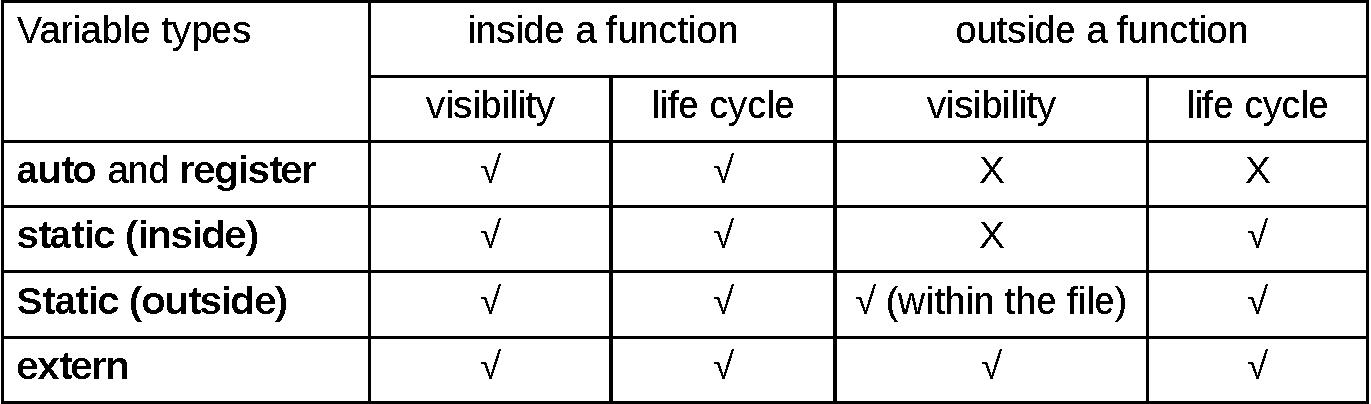
\includegraphics[width=0.8\linewidth]{figs/extern_var_eng.pdf}
\end{figure}
\begin{itemize}
	\item {It is NOT recommended to use global variables}
	\item {Advantage: you can transfer value easily}
	\item {Darkside}
	\begin{itemize}
		\item {You do NOT know where they have been changed}
		\item {Hard to debug your code}
		\item {Your code will be very messy!!!}
	\end{itemize}
\end{itemize}
\end{frame}